\documentclass{article}
\usepackage[utf8]{inputenc}
\usepackage{multirow}
\usepackage{graphicx}
\usepackage{subcaption}
\graphicspath{{./images/}{./confusion_matrices}}
\title{Project report classification MNIST database}
\author{Leik Lima-Eriksen and Torbjørn Bratvold}
\date{April 2020}

\begin{document}

\maketitle
\begin{abstract}

This project report describes the process of classifying the hand written numbers in the MNIST database\cite{MNIST} using two basic K nearest neighbour algorithms (KNN) and one template based KNN using clusters.  The two basic KNN used K = 1 and K = 4. Testing with 1000 hand written numbers The K = 4 KNN gave a lower error rate than the K = 1 KNN of $46\%$ verses $51.6\%$. Both had big problems classifying allot of none "one" numbers as the number "one". The classification time being $\approx1.4$ seconds per image (on the computer used). The template based KNN performed exept for the initial clustering  time (clustering can be done pre usage) much better for both error rate and classification time. The error rate was $\approx 4.8\%$ and the classifying time $\approx 0.14$ seconds per image. We confirmed that there is a linear relationship between the number of images to be classified and the processing time for all three classifiers. For the template KNN there seems to be some correlation between badly written numbers and wrongly classified numbers. There also seems to be a factor of randomness as some of the numbers are easily identified by a human.

\end{abstract}

\newpage
\tableofcontents
\newpage
\section{Introduction}
The project described in this report has the goal of classifying the handwritten numbers in the MNIST database\cite{MNIST}.
Three "k-nearest neighbour" algorithms are used to classify the images. Each classifier will be evaluated by performance and processing time.

Moving from the analog to the digital age a lot of literature and information are still stored on handwritten pages. Manually converting these pages to a digital searchable format takes allot of time and human resources. Automating this process would thus be a great leap towards giving people all over the world access to these sources. While we in this project only look at classifying numbers it is still an important step towards achieving this. It also has its standalone uses e.g. for answer sheets and written exams were only the input numbers are of interest.

\section{Theory}
\subsection{K-nearest neigbour}
The k nearest neighbour (KNN) algorithm has a simple decision rule were the input data is compared to a set of reference data. Reference data closest to the input data is then used to classify the input. \cite{Compendium in classification for TTT4275} In this implementation the reference and input data are n dimensional vectors were the euclidean distance between the input and a reference point is used to express similarity (smaller distance equals more similar).

The two first KNN algorithms used are quite straight forward. The first basic NN algorithm simply considers the single closest reference point to the input data for classification. While straight forward and easy to implement it is quite sensitive towards outliers.
The second algorithm considers a number "k" nearest reference points and uses a majority vote to classify the input. This gives more robustness towards outliers, but k must be carefully tuned as to large values will lead to local clusters being ignored.

The third and last uses a template version of the basic NN algorithm were $k = 1$, using clustered reference data for classification. Each reference class is arranged into a number "M" clusters. Each cluster is then represented by the average vector point and used as reference points for the NN algorithm. While harder to implement it gives robustness towards outliers and makes sure local clusters are accounted for. It will also perform better with large reference and input data-sets as the clusters can be calculated pre input and will thus consider a much smaller amount of references per input.

\subsection{K-means clustering}
While not going quite in dept, basic information about the cluster algorithm will be provided as it is quite essential for the NN template classifier. To create a number of M clusters the clustering is initialized by spawning M points in the coordinate system. The algorithm then follows iterations of two steps.
\begin{enumerate}

    \item All reference points are assigned to the closest spawned point and becomes a cluster.
    \item The spawned points are then re-spawned to the center of its corresponding cluster
\end{enumerate}
These two steps continue until convergence has been reached.

\subsection{Processing time}
For the two basic KNN algorithms each classification period uses the same amount of time and we should thus see a linear increase in processing time for the number of test images. We also expect the $K > 1$ algorithm to use a bit more time as it also need to do a majority vote.

For the template version the classification time should be significantly lower as it needs to consider fewer references than the two other versions. The clustering should take the most amount of time, but since it only needs to be done once the template version should have lower processing time for big test sets. We should also here see a linear increase in processing time as the number for tests increases and it will have a base processing time equal to the clustering time.


\section{Implementation}
The classifiers were implemented in python. To run the code you need to download the MNIST data-set from \cite{MNIST}, gunzip the files and put them into a directory named "mnist\_datasets". The directory must be in the same directory as the "mnist.py" file.


In figure \ref{fig:flow_1} and \ref{fig:flow_2} we see the flowcharts of the basic KNN and the template based KNN

\begin{figure}
\centering
\begin{minipage}[t]{.5\textwidth}
  \centering
  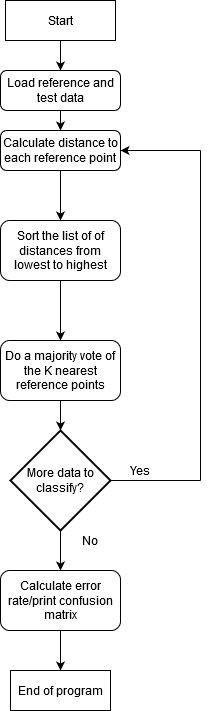
\includegraphics[scale=0.6]{images/flow_KNN.png}
  \captionof{figure}{Flowchart for the two basic KNN classifiers}
  \label{fig:flow_1}
\end{minipage}%
\begin{minipage}[t]{.5\textwidth}
  \centering
  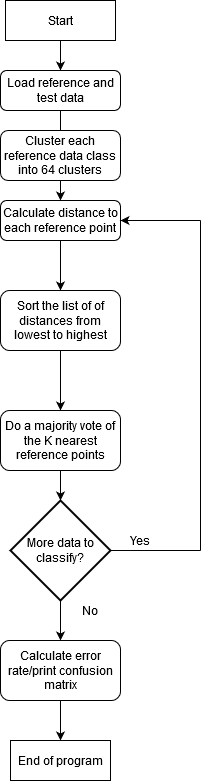
\includegraphics[scale=0.6]{images/cluster.png}
  \captionof{figure}{Flowchart for the templated based KNN classifier}
  \label{fig:flow_2}
\end{minipage}
\end{figure}



For clustering we used the function "KMeans" found in the sklearn library\cite{Kmeans}. It works by using the algorithm in 2.2. For calculating the euclidean distance between the reference and test points the function "scipy.spatial.distance.euclidean()" from the scipy library was used\cite{Scipy library}.
It calculates the distance using equation \ref{eq:dist}. Here d is the distance between the two vectors $u_i$ and $v_i$.
\begin{equation}
   d = \sqrt{\Sigma|(u_i-v_i)|^2}
   \label{eq:dist}
\end{equation}
We also used the numpy library for its arrays and fast operations \cite{Python library Numpy}

\newpage

\section{Results}
\begin{table}[]
\centering
\begin{tabular}{lllll}
\hline
\multicolumn{1}{|l|}{\multirow{3}{*}{Images classified}} & \multicolumn{4}{l|}{KNN}                                                                                                            \\ \cline{2-5}
\multicolumn{1}{|l|}{}                                   & \multicolumn{2}{l|}{K = 1}                                       & \multicolumn{2}{l|}{K = 4}                                       \\ \cline{2-5}
\multicolumn{1}{|l|}{}                                   & \multicolumn{1}{l|}{Time used} & \multicolumn{1}{l|}{Error rate} & \multicolumn{1}{l|}{Time used} & \multicolumn{1}{l|}{Error rate} \\ \hline
\multicolumn{1}{|l|}{100}                                & \multicolumn{1}{l|}{132.2s}    & \multicolumn{1}{l|}{36.0\%}     & \multicolumn{1}{l|}{137.8s}    & \multicolumn{1}{l|}{33.0\%}     \\ \hline
\multicolumn{1}{|l|}{1000}                               & \multicolumn{1}{l|}{1354.8s}   & \multicolumn{1}{l|}{51.6\%}     & \multicolumn{1}{l|}{1474.3s}   & \multicolumn{1}{l|}{46.0\%}     \\ \hline
                                                         &                                &                                 &                                &                                 \\ \hline
\multicolumn{1}{|l|}{\multirow{3}{*}{Images classified}} & \multicolumn{4}{l|}{Cluster NN}                                                                                                     \\ \cline{2-5}
\multicolumn{1}{|l|}{}                                   & \multicolumn{2}{l|}{Clustering}                                  & \multicolumn{2}{l|}{Classifying}                                 \\ \cline{2-5}
\multicolumn{1}{|l|}{}                                   & \multicolumn{2}{l|}{Time used}                                   & \multicolumn{1}{l|}{Time used} & \multicolumn{1}{l|}{Error rate} \\ \hline
\multicolumn{1}{|l|}{100}                                & \multicolumn{2}{l|}{327.5s}                                      & \multicolumn{1}{l|}{1.4s}      & \multicolumn{1}{l|}{5.0\%}      \\ \hline
\multicolumn{1}{|l|}{1000}                               & \multicolumn{2}{l|}{364.5s}                                      & \multicolumn{1}{l|}{14.8s}     & \multicolumn{1}{l|}{4.8\%}      \\ \hline
\multicolumn{1}{|l|}{10000}                              & \multicolumn{2}{l|}{360.7s}                                      & \multicolumn{1}{l|}{127.3s}    & \multicolumn{1}{l|}{4.5\%}      \\ \hline
\end{tabular}
\caption{Processing time and error rates of the KNN classifiers}
\label{tbl:time}
\end{table}

In table \ref{tbl:time} we can see the processing time and error rate for the three classifiers. The processing time was calculated on a laptop running windows, therefor the time may vary when calculated on other computers, the ratios should however stay roughly the same. The two non template KNN classifiers were not tested with 10000 test images as it would take far to long to process. For these two we can see the the ratio between time used and number of images are almost the same for both $100$ and $1000$ tested images. The error rate increases as more images were tested. For 100 tests KNN with K = 4 has an error rate that is $3\%$ lower than for K = 1. For 1000 tests the difference increases and becomes 4.6\% lower for K = 4

The clustering is clearly the most effective algorithm. The processing time for classification is about 100 times lower than for the non template classifiers. While the clustering uses around 350 seconds to complete, it is relatively constant for both amounts of test data. For an amount of test data over ca. 260 samples the template version will use a lower total time with clustering included.

The error rate of the template classifier for 1000 tests is only $4.8\%$ which is nearly 10 times lower than for the K = 4 NN.
From the confusion matrixes in figures \ref{fig:NN_1000}-\ref{fig:ckustr_1000}  we can see that the template NN is in general not biased towards any specific number while the two KNN have a large amount of numbers mislabeled as "one".
\newline
\begin{figure}[htbp]
  \centering
  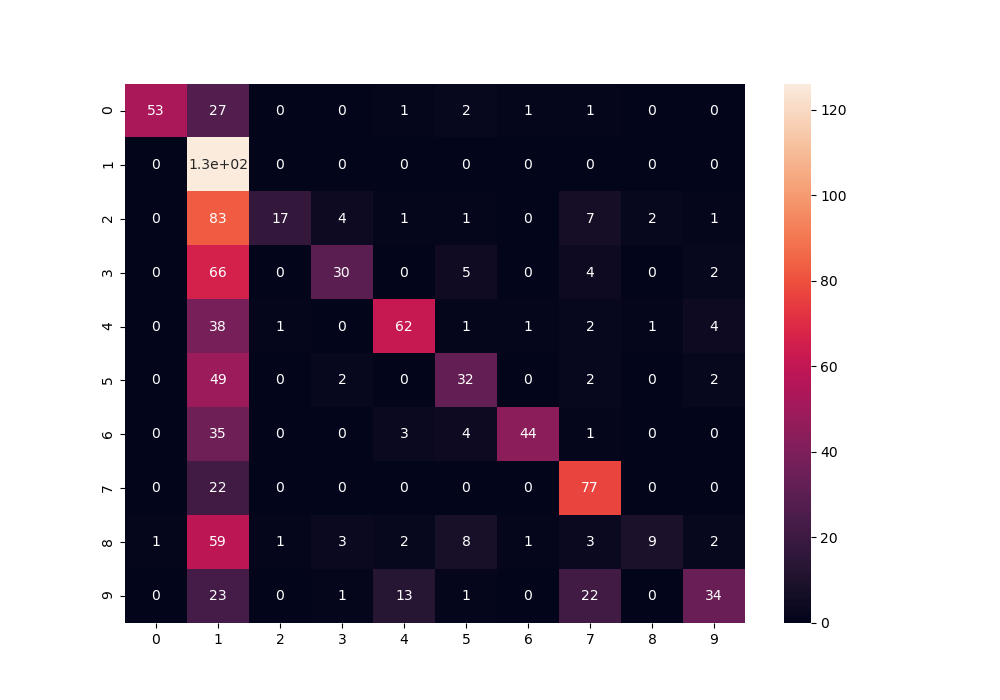
\includegraphics[width=\textwidth]{./confusion_matrices/NN_1000.png}
  \caption{K = 1 NN, 1000 test samples}
  \label{fig:NN_1000}
\end{figure}

\begin{figure}[htbp]
  \centering
  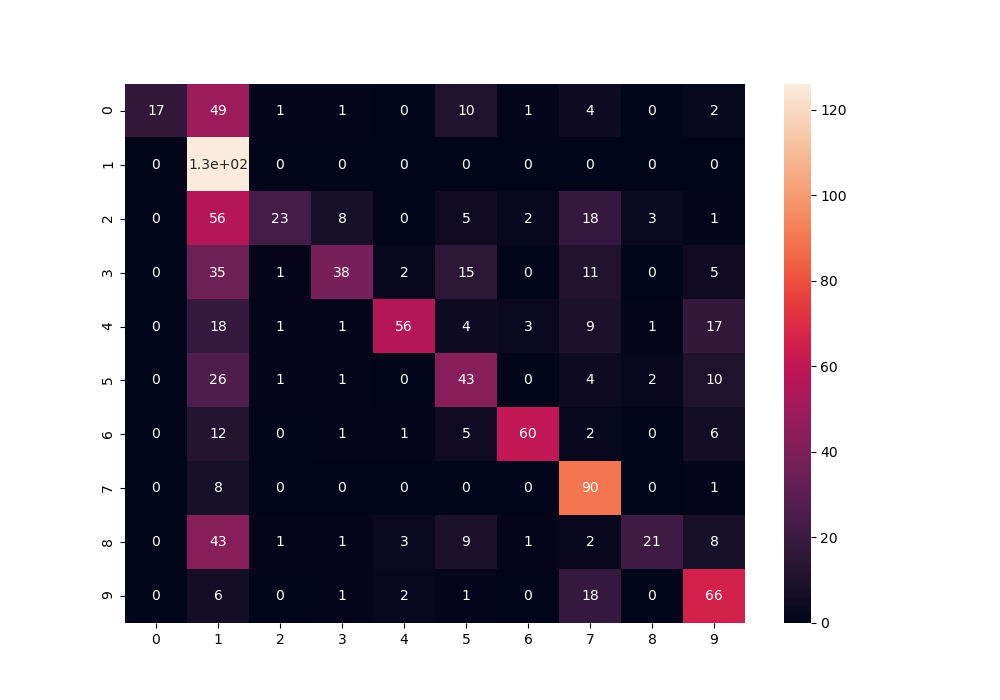
\includegraphics[width=\textwidth]{./confusion_matrices/KNN4_1000.png}
  \caption{K = 4 NN, 1000 test samples}
  \label{fig:KNN_1000}
\end{figure}

\begin{figure}[htbp]
  \centering
  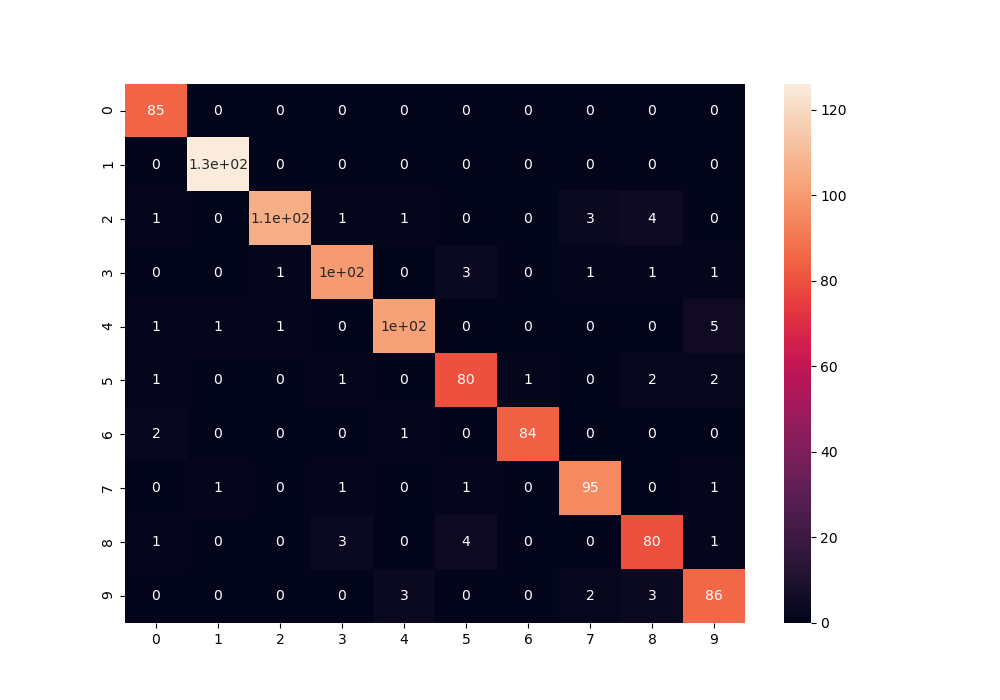
\includegraphics[width=\textwidth]{./confusion_matrices/Cluster_1000.png}
  \caption{Template NN using clustering, 1000 test samples}
  \label{fig:ckustr_1000}
\end{figure}

In figure \ref{fig:right} and \ref{fig:wrong} we see some of the correctly and miss-correctly labeled numbers of the template KNN classifier. Here T is the correct number and P is the number predicted by the classifier. The numbers in \ref{fig:wrong} are quite ordinary and should pose no problem for a human to identify. In figure \ref{fig:right} some of the numbers can be harder to read. Especially the 5 in the second row from the top and the number 3 in the bottom row. While other again seem completely normal like the 5 in the second bottom row and the 0 in the second top row. This indicate that while there is some correlation between badly written numbers and the classifiers inability to predict them correctly, there also seem to be an aspect of randomness involved.

\begin{figure}
\centering
\begin{minipage}[t]{.5\textwidth}
  \centering
  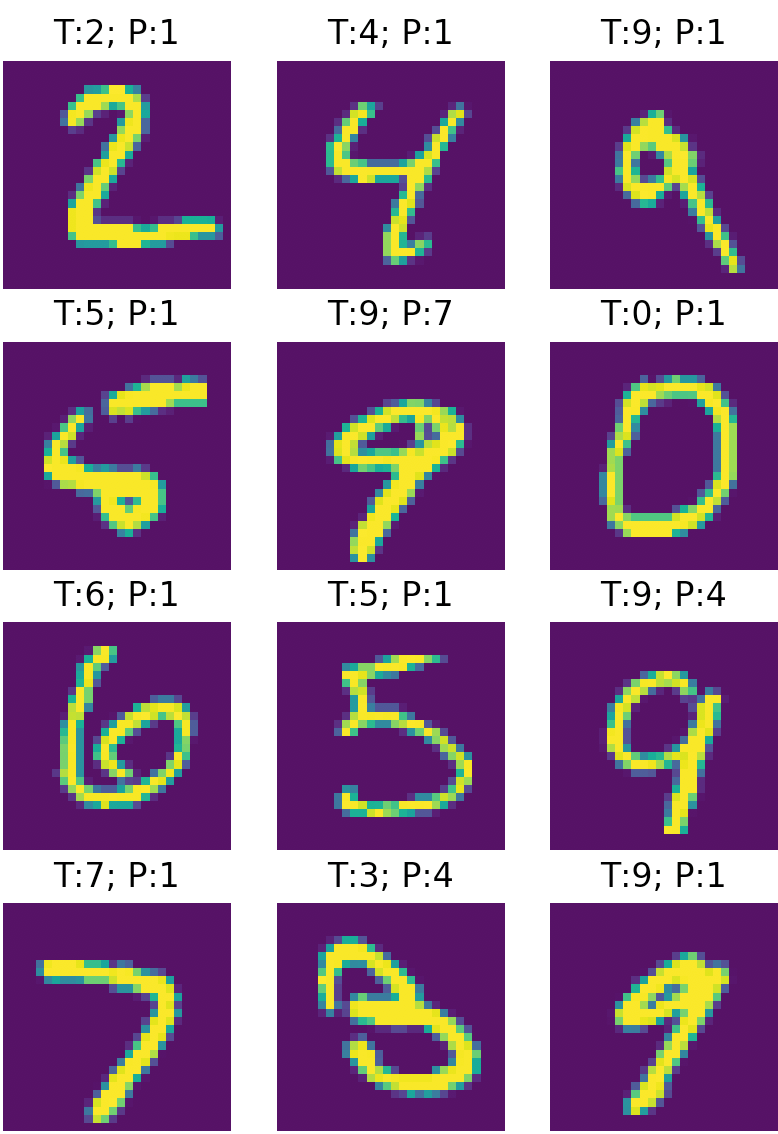
\includegraphics[width=0.9\linewidth]{images/correct_class.png}
  \captionof{figure}{Pictures of correctly classified numbers using template KNN}
  \label{fig:right}
\end{minipage}%
\begin{minipage}[t]{.5\textwidth}
  \centering
  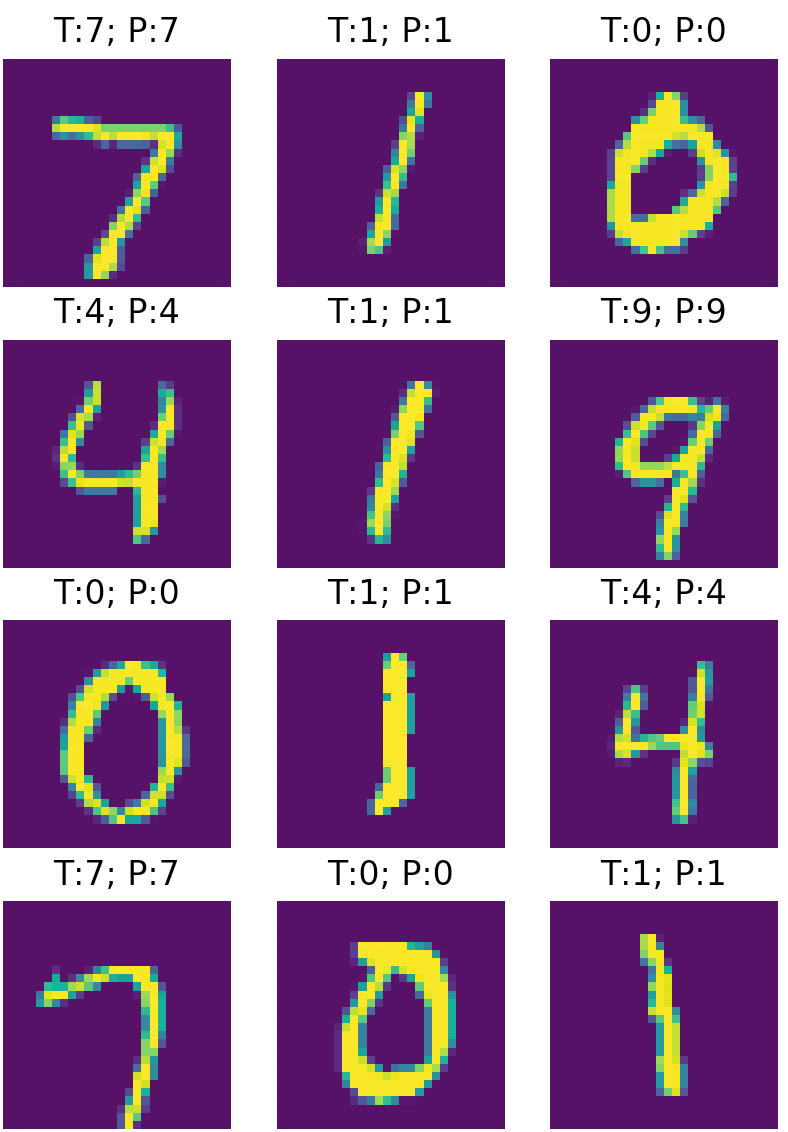
\includegraphics[width=0.9\linewidth]{images/wrong_class.png}
  \captionof{figure}{Pictures of wrongly classified numbers using template KNN}
  \label{fig:wrong}
\end{minipage}
\end{figure}

\newpage

\section{Discussion}
As predicted in the theory part 2.3 the classifiers show a linear trend in processing time as the number of test data increases. While the classification of a single image is fast enough for real-time usage for all three classifiers the template version is clearly superior in both time and error rate. It should be used for all purposes were a low error rate is important or when clustering can be utilized before test data is inputted. The error rate of the two non template KNN classifiers are so high that they are probably not usable without being heavily monitored.
We also see a large discrepancy in error rate between a 100 and a 1000 test images. This is probably from a 100 test samples not being large enough to correctly estimate the true error rate of the classifier thus an error rate of around 50\% will be more in line for standard use.
The main error factor as shown in the confusion matrixes in figures \ref{fig:NN_1000}-\ref{fig:ckustr_1000} comes from other numbers being miss-classified as "one". If the number "one" is not used as reference or for testing the two non template KNN might give a lower error rate than they currently do. This should be looked into before a possible use.

\section{Conclusion}
As discussed in the theory part the classifiers had a linear increase in processing time in relation to the amount of test data. The K = 1 and K = 4 KNN classifiers had an error rate of about $51.6\%$ and $46\%$ respectively. The lower error rate for K = 4  The time to classify a single number was $\approx 1.35$ second with marginally higher processing time for K = 4 .
While the template based NN classifier is initially slower because of the clustering time of $\approx 350$ seconds, the classifying itself has a speed of $\approx 0.14$ seconds per number which is $\approx 100$ times faster than the two basic KNN classifiers. The clustering can be performed pre classifying and should thus not add to any real-time processing. The template error rate was also superior with an error rate of $\approx 4.8\%$ for all number of test data. Here the wrongly predicted numbers seem to have some correlation with how badly they are written, but some of the miss-predicted numbers are easily identified by a human eye. Thus it seems there is also an aspect of randomness involved for the miss-predicted numbers.
The two non template KNN classifiers had a big tendency to miss-classify other numbers as "one". For these to be used in any viable way one should evaluate their performance when the number "one" is not part of the reference or test data.

\begin{thebibliography}{99}
\bibitem{Compendium in classification for TTT4275}

  Magne H. Johnsen., December 18, 2017, \emph{TTT4275- Estimation, detection and classifying
: Compendium in classification for TTT4275}
\bibitem{Kmeans}
scikit-learn developers., April 2020, \emph{https://scikit-learn.org/stable/modules/generated/sklearn.cluster.KMeans.html}

\bibitem{Python library Numpy}
NumPy developers., April 2020, \emph{https://numpy.org/index.html}

\bibitem{Scipy library}
The SciPy community,. April 2020

\emph{https://docs.scipy.org/doc/scipy/reference/generated/scipy.spatial.distance.euclidean.html}

\bibitem{MNIST}
Yann LeCun, Professor
The Courant Institute of Mathematical Sciences, Corinna Cortes, Research Scientist
Google Labs, New York,
New York University,. April 2020
\emph{http://yann.lecun.com/exdb/mnist/}
\end{thebibliography}


\end{document}

